\documentclass[12pt,paper=A4,numbers=noenddot,bibliography=totoc,listof=totoc,DIV=11,BCOR=1mm]{scrreprt}

\usepackage[T1]{fontenc}
\usepackage[english]{babel}
\usepackage[utf8]{inputenc}
%-----------------------------------------
\usepackage{blindtext}
%-----------------------------------------
%\setlength{\textwidth}{}
%\setlength{\textheight}{}
%\setlength{\oddsidemargin}{}
%\setlength{\topmargin}{} 
\usepackage{booktabs}
\usepackage{graphicx}
\usepackage{geometry}
\usepackage[dvipsnames]{xcolor}
\usepackage{amsmath}
\definecolor{dunkel}{cmyk}{1,.60,0,.40}
\definecolor{gdunkel}{cmyk}{1,.80,0,.60}
\definecolor{hell}{cmyk}{.28,.12,0,.15} 
\definecolor{ghell}{cmyk}{.14,.06,0,.08}
\definecolor{lightgray}{rgb}{0.83, 0.83, 0.83}
\definecolor{mygray}{gray}{0.3}

%%%%%%%%%%%%%%%%%%%%%%%%%%%%%%%%%%%%%%%% Program Code %%%%%
\usepackage{listings}
%\usepackage{minted}
%\usepackage{xcolor}
\usepackage{adjustbox}
\usepackage{verbatim}
\definecolor{shadecolor}{rgb}{.9, .9, .9}

\newenvironment{code}%
   {\par\noindent\adjustbox{margin=1ex,bgcolor=shadecolor,margin=0ex \medskipamount}\bgroup\varwidth\linewidth\verbatim}%
   {\endverbatim\endvarwidth\egroup}

\newenvironment{code2}%
   {\par\noindent\adjustbox{margin=1ex,bgcolor=shadecolor,margin=0ex \medskipamount}\bgroup\minipage\linewidth\verbatim}%
   {\endverbatim\endminipage\egroup}
%%%%%%%%%%%%%%%%%%%%%%%%%%%%%%%%%%%%%%%%%%%%%%%%%%%%%%%%%%%%%%%%%

\definecolor{codegreen}{rgb}{0,0.6,0}
\definecolor{codegray}{rgb}{0.5,0.5,0.5}
\definecolor{codepurple}{rgb}{0.58,0,0.82}
\definecolor{backcolour}{rgb}{0.95,0.95,0.92}

\lstdefinestyle{mystyle}{
    backgroundcolor=\color{backcolour},   
    commentstyle=\color{codegreen},
    keywordstyle=\color{magenta},
    numberstyle=\tiny\color{codegray},
    stringstyle=\color{codepurple},
    basicstyle=\ttfamily\footnotesize,
    breakatwhitespace=false,         
    breaklines=true,                 
    captionpos=b,                    
    keepspaces=true,                 
    numbers=left,                    
    numbersep=5pt,                  
    showspaces=false,                
    showstringspaces=false,
    showtabs=false,                  
    tabsize=2
}

\lstset{style=mystyle}

%%%%%%%%%%%%%%%%%%%%%%%%%%%%%%%%%%%%%%%%%%%%%%%

\usepackage{hyperref}
\hypersetup{
    colorlinks=true,
    linkcolor=blue,
    filecolor=magenta,      
    urlcolor=cyan,
}
\urlstyle{same}

%%%% own shortcuts %%%%
\newcommand{\bild}[3]{%
	\begin{figure}[htbp]
	\begin{center}
	\includegraphics[width=0.8\textwidth]{bilder/#1}
	\caption{#3}\label{#2}
	\end{center}
	\end{figure}
}
\newcommand{\bildscaled}[4]{%
	\begin{figure}[htbp]
	\begin{center}
	\includegraphics[scale=#4]{bilder/#1}
	\caption{#3}\label{#2}
	\end{center}
	\end{figure}
}
%%%%%%%%%%%%%%%%%%%%%%%%%%%%%%%%%%%%%

\usepackage[round,authoryear]{natbib}
\bibpunct[:\,]{(}{)}{,}{a}{}{,~}

%%%%%%%%%%%%%%%%%%%%%%%%%%%%%%%%%%%%%

\begin{document}

\begin{titlepage}
\newgeometry{left=5.5cm} %defines the geometry for the titlepage
\pagecolor{dunkel}
\noindent
\hspace*{-3mm}
\includegraphics[width=10em]{titlepagestuff/bild4}\\[-1.2em]
\color{white}
\makebox[0pt][l]{\rule{1.3\textwidth}{1pt}}
\par
\noindent
\makebox{%
\small\textbf{\textsf{Faculty Design, Orbital Mechanics and Aviation}} \hspace{0.3ex} \textcolor{hell}{\textsf{Department Science}}}

\normalsize 
\vspace{20mm}
\noindent
\textsf{\LARGE Master's Thesis}\\[0.4ex]
\textsf{\small In Partial Fulfillment of the Requirements for the Degree of M.Sc.}
%\textsf{\small In Partial Fulfillment of the Requirements for the Degree of\\Master of Science (M.Sc.)}

\vspace{5mm}
\noindent
\textsf{\LARGE Max Kerman}\\ \textsf{\small Matr.-Nr. 3141592}

\vspace{15mm}
\noindent
{\huge\textsf{CommNet Kerbin System}}

\vspace{5mm}
\noindent
{\Large\textsf{A web of three relay satellites per body\\ to ensure a full coverage of the Kerbin system}}


\vfill
\noindent
\textsf{\large%
first examiner: Seb Kerman\\
second examiner: Valentina Kerman
}

\vspace{3mm}
\noindent
\textsf{\large \today}
\end{titlepage}
\restoregeometry % restores the geometry
\nopagecolor % Use this to restore the color pages to white
%%%%%%%%%%%%%%%%%%%%%%%%%%%%%% 

%\maketitle

\tableofcontents

\chapter{Kerbin Satellites}

\bildscaled{Kerbin}{kerbin}{Kerbin Relay Network}{0.5}

We want to create a communications network with three equally distanced satellites in an equatorial orbit around planet Kerbin. There is a simple reason for this:

For the control of a spaceship, a space station or a satellite we usually need an active connection to the Kerbal Space Center (KSC).
But by positioning three equally distanced satellites in the same orbit around the planet, we can prevent the connection getting cut off as soon as the KSC disappeares behind the horizon. Algorithms will automatically choose the shortest connection using as few satellites as possible.

Kerbin is a relatively small planet. Kerbin's 600km radius measures just one tenth of the radius of planet Earth. Also the game won't calculate transmission time delays (\href{https://www.wikiwand.com/en/Latency_(engineering)}{Latency}), which is why we only need to ensure that the connection holds, not how good it actually is. Another point is that we want to enable interplanetary communication with our CommNet. So we want to choose a higher antenna strength than necessary for a communication between our three satellites. In order to survey as much as possible from the round planet’s surface (just think about the difficulty of reaching the poles), we will set the satellites into a high orbit. The greater the distance between the sphere and the observer, the larger the visible surface gets.

However, if we wanted to create a internet network, the way SpaceX does with Starlink, then a lower orbit would be much more favourable in order to shorten the latency. But this would require much more satellites per orbit, as the communication would otherwise have to go through the planet's surface, which isn't possible after all. The satellites must be at least high enough to see each other just above the horizon.

We choose an equatorial orbit, mainly because it will require less fuel and therefore less weight for the rocket. Also the Kerbal Space Center lies directly at the equator, hence one must only ``fall'' to the east to get into orbit. In addition, the rotation of the earth will give a small boost to the rocket, as it doesn't need to create this starting speed by itself. On average, you will save about \href{https://wiki.kerbalspaceprogram.com/wiki/Kerbin}{175m/s}.

From experience the loss of speed resulting from atmospheric drag will be about 1000m/s. More precise calculations are neither worthwhile nor possible for that matter, as the game only simulates the impact of the surrounding air. For a western start one should also calculate an additional 300m/s. For further details, see the Youtube video by Mike Aben \href{https://youtu.be/0BtbYVtZ9ac}{Ascent Costs of Inclined Orbits - KSP Let's Do The Math}.

If you have the ground stations on Kerbin deactivated, you won't be able to control the rocket anymore as soon as the KSC loses sight. You can either activate the ground system and keep it switched on, until your own satellite system is in operation, or you keep it off and use a kOS-script to release the satellites (more on that later).

Should you already have some space junk, with the capacity to communicate flying around from previous failed attempts, then you can just use those as a temporary replacement for a proper network.


\section{Target Orbit}
The target orbit ought to be high enough so that you could draw a straight line from one satellite to another without it touching the planet's surface. However, the target orbit should not be too high so not to leave the sphere of influence (SOI) of the planet and sail away into infinity. The best orbit height lies somewhere in between. There is also a specific satellite orbit, wherein a complete rotation around the planet takes up the same amount of time as it does for the planet to rotate around it’s own axis(i.e. One Day). Thereby a person standing on the surface of the planet would view the satellite as if it was standing still. The correct term for this kind of orbit is ``synchronous orbit''.

The \href{https://wiki.kerbalspaceprogram.com/wiki/Kerbin}{KSP Wiki} states $2863.334km$ as the height of a synchronous orbit. This means that all objects in this orbit need 5h 59m 9.4s for one complete rotation around the planet.


\subsection{Alternative Orbit}
\href{https://youtu.be/PZAkiXNJIqc}{Tipp: Geostationary, Molniya, Tundra, Polar \& Sun Synchronous Orbits Explained - Scott Manley}\\
If you still want a different orbit, then you will have to deal with a little bit of geometry ;)

First we calculate the lowest possible orbit for our chosen number of satellites.
The orbit height from the planet's center (radius \emph{r}) we get through this formular:
\begin{equation}
r_{orbit} = \frac{r_{planet}}{\sin \frac{\theta}{2}}
\end{equation}
The angle $\theta$ of the polygon is being calculated by:
\begin{equation}
\theta = \frac{(n-2) \cdot 180^{\circ}}{n}
\end{equation}
$(n-2) \cdot 180^{\circ}$ stands for the sum of angles from the regular polygon and
\emph{n} for the number of angles, or rather for the number of satellites in orbit.
In our case we have a triangle $\rightarrow$ so $\theta = 60^{\circ}$ for each of the three interior angles.
$$
r_{orbit} = \frac{r_{planet}}{\sin \frac{\theta}{2}} = \frac{600km}{\sin \frac{60^\circ}{2}} = 1200km
$$
For us this means that we have got a $1200km - 600km = 600km$ distance from the surface of the planet for the lowest possible orbit that one can achieve with three satellites at the equator.

As time goes by the satellites will slightly change their position between each other, provided that they aren't being maintained or the safefile isn't being manipulated: \href{https://youtu.be/0wXVm3M2I2w}{Kerbal Space Program - Savefile Editing \& Orbital Parameters Tutorial (Fixed) - Scott Manley}.
This means that sooner or later the connection between the satellites will be interrupted by the surface of the planet. For this reason it's advisable to add a small buffer of about a few kilometers to a low orbit.


\medskip The orbital period of the target orbit (final orbit) is obtained by:

\begin{equation}
T_{f} = 2\pi \sqrt{\frac{a_{f}^{3}}{\mu}} = 2\pi \sqrt{\frac{(1200km)^{3}}{\mu}} = 4395s
\end{equation}

\begin{flushright}
$\mu = 3.5316 \cdot 10^{12} \frac{m^{3}}{s^{2}} = 3531.6 \frac{km^{3}}{s^{2}}$ \\
(Kerbin standard gravitational parameter)
\end{flushright}
\begin{flushright}
In a circular orbit, the semimajor axis \emph{a}\\ is equal to the orbit radius \emph{r}, the periapsis \emph{Pe} and the apoapsis \emph{Ap}.
\end{flushright}

\medskip But back to the ``synchronous orbit''.

\section{Transfer Orbit}
Now the question is how to actually deploy the satellites into their orbit while at the same time spacing them at equal distances.
The Youtuber ``Stratzenblitz75'' has made a great video on this topic.
\href{https://youtu.be/3Qb_gcJyGQI}{KSP/RSS - Building a Comm Network with Math! - [Stratlab EP1]} \href{https://en.wikipedia.org/wiki/Geostationary_transfer_orbit}{, GTO = geosynchronous / geostationary transfer orbit}

We measure (or calculate) the time a satellite spends in the target orbit for one complete rotation around the planet. That time is also called ``orbital period''. In our case we already know from the KSP Wiki that the orbital period is about 6 hours which is the same as one Kerbin Day.
And we want to release three equally distanced satellites in this orbit. This means that each satellite has a temporal distance of 2 hours (1/3 of it's orbit) to the next one.

The next thought would possibly be to just release the satellites one after the other at the same spot in the target orbit. The released satellite will of course then fly on in it's orbit and make place for the next one. If we play our cards right, then we will release the next satellite only after the former one has completed a distance of exactly 1/3 of it's orbit.

This, in turn, is possible by first putting all three satellites onto one single rocket, which will then pass the exact spot periodically.
The orbit of the rocket must have the form of an ellipse. The highest part of the orbit is called apoapsis and is exactly the one that passes the target orbit. The lowest part of the orbit is called periapsis (you will also hear things like apogee or perigee) and has been deliberately chosen to make the orbital period exactly 2/3 of the target orbit.
Now, everytime the rocket passes it's apoapsis, a new satellite will be released.
After three full cycles, all the satellites will hopefully have been deployed. Now the rocket can begin it's deorbit burn to lower it's periapsis and to burn up in the atmosphere and simultaneously reduce space debris. This is done for safety reasons, but in KSP it primarily improves the runtime performance, as less parts will have to be rendered. Because the population density on Kerbin is very low, it isn't a problem to crash your parts into the planet, but in real life you would try to make sure that the parts burn up in the atmosphere before hitting the ground.
Alternatively there is also a button inside the KSC Observation Center to delete those parts.

If, however, the lowest part of this transfer orbit goes through the surface of the planet (precisely because the target orbit is set so low), then we can just change it's orbital period to something, that isn't 2/3 but rather 5/6 of the target orbit.
This will hopefully place the periapsis above the planet's surface (and it's atmosphere).
However it should be noted that in order to reach the goal, now we can only release one satellite every two cycles around the planet, instead of every round with a 2/3 orbit.
In this case the orbital period ammounts to $5/6 \cdot 6h = 5h$.

If, at this point the lower part of this orbit is still too close to the planet, then we can decide to choose a 4/3 orbit. This way the periapsis will be at the height of the target orbit and the apoapsis higher than that. In this case the orbital period ammounts to $4/3 \cdot 6h = 8h$.

The closer the transfer orbit is to the target orbit, the better. The satellite will have to spend less energy to get into it's final orbit. This in turn leads to a smaller satellite, as less fuel (and thrust) will be needed.\\

But where do we now put the transfer orbit? All that is needed are the apoapsis and the periapsis. We already got one of the two. That's the point where the transfer orbit intersects the target orbit. We can now calculate the other point with the help of the orbital period:
\bildscaled{i_orbit}{i_orbit}{Transfer Orbit Parameter}{0.7}
\pagebreak 
\begin{flushleft}
Orbital\,Period\,from\,the\,Transfer\,Orbit:
\end{flushleft}
%\begin{eqnarray}
%T_{i} &=& \frac{2}{3}T_{f}\\
%      &=& \frac{2}{3} \cdot 6h\\
%      &=& ...s
%\end{eqnarray}
\begin{equation} \label{eq1}
\begin{split}
T_{i} &= \frac{2}{3}T_{f} \\
      &= \frac{2}{3} \cdot 6h \\
      &= 14400s
\end{split}
\end{equation}
\begin{center}
Or how the KSP Wiki states it:\\
$T_{f} = 5h\,59m\,9.4s = 21549.425s$ \\
$T_{i} = \frac{2}{3} \cdot 21549.425s = 14366.283s$
\end{center}

\begin{flushleft}
Semimajor Axis from the Transfer Orbit:
\end{flushleft}
\begin{equation}
\begin{split}
a_{i} &= \sqrt[3]{\frac{\mu \cdot T_{i}^{2}}{4\pi^{2}}} \\
   &= \sqrt[3]{\frac{3531.6 \frac{km^{3}}{s^{2}} \cdot (14366.283s)^{2}}{4\pi^{2}}} \\
   &= 2643km
\end{split}
\end{equation}

\begin{flushleft}
Periapsis from the Transfer Orbit:
\end{flushleft}
\begin{equation}
\begin{split}
Pe &= 2a_{i} - Ap \\
   &= 2(2643km) - (600km + 2863.334km) \\
   &= 1822.7km
\end{split} 
\end{equation}
Here, the orbit height amounts to $1822.7km - 600km = 1222.7km$ above the surface.

\bigskip
Alternatively you could of course just use the online \href{https://meyerweb.com/eric/ksp/resonant-orbits/}{Resonant Orbit Calculator} by Eric Meyer. After choosing the planetary body the calculator will present you with the required $\Delta v$ for each satellite. Especially the visual presentation helps in the understanding.

\section{Delta-v budget of each satellite}
$\Delta v$ can be understood as the whole change in velocity without the influence of drag and other parameters. If we were to simply separate the satellite from it's rocket then it might move away a little bit, but the orbit would stay more or less the same. To finally get into the target orbit, the satellite must first burn prograde (in the moving direction) at the apoapsis until it's velocity is as high as are all objects inside of the target orbit. For our ``synchronous orbit'' this would mean a velocity of $v = \sqrt{\frac{\mu}{r_{o}}} = 1110m/s$ for every object in this orbit, whereby $r_{o}$ must be the radius of a round orbit. The higher the orbit, the higher the potential energy and the lower the speed. Or \href{https://en.wikipedia.org/wiki/Kepler%27s_laws_of_planetary_motion}{2. Kepler's law}: ``A line segment joining a planet and the sun sweeps out equal areas during equal intervals of time.''. Objects in a lower orbit must therefore move faster.\\

How much $\Delta v$ does the satellite need to get from the transfer orbit to the target orbit?
For this purpose we use the \hyperlink{visviva}{Vis-Viva Equation}:

\begin{equation*}
\begin{split}
\Delta v_{2} &= \sqrt{\frac{\mu}{r_{2}}} \left( 1-\sqrt{\frac{2r_{1}}{r_{1}+r_{2}}} \right) \\
             &= \sqrt{\frac{3531.6 \frac{km^{3}}{s^{2}}}{3463.334km}} \left( 1-\sqrt{\frac{2(1822.7km)}{1822.7km+3463.334km}} \right) \\
             &= 0.171224\frac{km}{s} \\
             &= 171.224\frac{m}{s}
\end{split}
\end{equation*}
\begin{flushright}
$r_{1} = 1822.7km = Pe$ \\
$r_{2} = 3463.334km = Ap$
\end{flushright}

\section{Delta-v budget of the rocket}
\href{https://youtu.be/aSH07ngBbIY}{Ascent \& Injection Costs - KSP Let's Do The Math \#6}\\
\href{https://youtu.be/0BtbYVtZ9ac}{Ascent Costs of Inclined Orbits - KSP Let's Do The Math \#7}\\

The rocket will execute three burn maneuvers:
\begin{enumerate}
\item Start from the surface of Kerbin, until the apoapsis is 1822.7km (1222.7km above ground).
\item Orbit circularisation burn at the apoapsis to raise the periapsis to the same height.
\item Raising the apoapsis to the height of the target orbit at 3463.334km (2863.334km above ground).
\end{enumerate}
Of course one can also achieve the same with only two maneuvers, but then the accuracy would suffer. In addition one would waste a lot of fuel, because the longer the burn, the less the time at which the rocket will actually burn into the prograde direction.

\begin{flushleft}
Sidereal rotational velocity of Kerbin: $\overrightarrow{v_{r}} = 174.94 m/s$ \\
Air drag by experience: $\overleftarrow{drag} = 1000 m/s$ \\
Radius of Kerbin: $r_{1} = 600km$ \\
Radius from the first preliminary orbit: $r_{2} = 1822.7km$ \\
Radius from the target orbit: $r_{3} = 3463.334km$
\end{flushleft}

Let's now calculate the necessary energy for the first level:

\begin{equation*}
\Delta v_{1} = \sqrt{\frac{\mu}{r_{1}}} \left( \sqrt{\frac{2r_{2}}{r_{1}+r_{2}}}-1 \right)
             = 549.89 m/s
\end{equation*}
\begin{equation*}
\Delta v_{2} = \sqrt{\frac{\mu}{r_{2}}} \left( 1-\sqrt{\frac{2r_{1}}{r_{1}+r_{2}}} \right)
             = 412.3 m/s
\end{equation*}
\begin{equation*}
\Delta v_{1} = \sqrt{\frac{\mu}{r_{2}}} \left( \sqrt{\frac{2r_{3}}{r_{2}+r_{3}}}-1 \right)
             = 201.4 m/s
\end{equation*}

\begin{flushright}
\begin{tabular}{c@{\,}c@{\,}c@{\,}c@{\,}c@{\,}c@{\,}c@{\,}c}
  & 5 & 4 & 9 & . & 8 & 9 \\ 
+ & 4 & 1 & 2 & . & 3 &   \\ 
+ & 2 & 0 & 1 & . & 4 &   \\ 
\hline 
1 & 1 & 6 & 3 & . & 5 & 9 \\ 
\end{tabular}
\end{flushright}

Until now we pretended that the rocket will start from an orbit with the height of 600km. But of course the rocket starts actually from the ground's surface with the speed of the planet's own rotation.
Thus, we still need the necessary velocity for an orbit of 600km, plus the speed which was lost due to air drag inside the atmosphere, minus the additional rotation speed of the planet at a launch to the east.\\

\begin{flushleft}
Theoretical orbital velocity at ground level:
\end{flushleft}
\begin{equation*}
\Delta v = \sqrt{\frac{\mu}{600km}} = 2426.1 m/s
\end{equation*}
\begin{flushright}
\begin{tabular}{c@{\,}c@{\,}c@{\,}c@{\,}c@{\,}c@{\,}c@{\,}c}
  & 2 & 4 & 2 & 6 & . & 1 &   \\ 
+ & 1 & 0 & 0 & 0 &   &   &   \\ 
- &   & 1 & 7 & 4 & . & 9 & 4 \\ 
\hline 
  & 3 & 2 & 5 & 1 & . & 1 & 6 \\ 
\end{tabular}
\end{flushright}
\hypertarget{kerbinrocketdrag}{Therefore the rocket requires a minimum $\Delta v$ of}
$$
1163.59 m/s + 3251.16 m/s = \mathbf{4414.75 m/s}.
$$
If you really want to fly as economically as possible, then you should start with the very lowest possible orbit above the atmosphere, somewhere in between 70-80km. From there on you should raise the apoapsis ``directly'' to the height of the target orbit. After arriving at the apoapsis, the rocket should then raise it's periapsis for the correct transfer orbit.

In this case you optimally want to raise the orbit only incrementally by using the so-called ``orbit phasing'' method, just as Rocket Lab does it with it's \href{https://youtu.be/zC8RxgL9tK4?t=680}{Photon} Kick Stage on it's way to the moon.
\bildscaled{orbit_phasing}{orbit_phasing}{Orbit Phasing Maneuver}{1.0}


\chapter{Mun Satellites}
Mun is the closest neighbor to Kerbin. Strong antennas are therefore less relevant than a continuous communication connection with the vessels that might lie inside the mun shadow as seen from Kerbin (behind Mun). In the worst case scenario, a loss of connection will lead to a complete loss of control. This is particularly relevant if you want to land on the moon's surface.\\

Because the approach does not differ much from the one used on the Kerbin satellites, I won't go into detail as much.
\medskip
\begin{flushright}
\href{https://wiki.kerbalspaceprogram.com/wiki/Mun}{Mun Properties:} \\
Equatorial radius $ = 200km$ \\
$\mu = 6.5138398 \cdot 10^{10} \frac{m^{3}}{s^{2}} = 65.1384 \frac{km^{3}}{s^{2}}$ \\
SOI (Sphere of influence) $ = 2429.5591 km$
\end{flushright}
\bildscaled{Mun}{mun}{Mun Relay Network}{0.5}
\pagebreak 
\begin{flushleft}
Minimal Orbit:
\end{flushleft}
\begin{equation*}
r_{orbit} = \frac{r_{mun}}{\sin \frac{\theta}{2}} = \frac{200km}{\sin \frac{60^\circ}{2}} = 400km
\end{equation*}
$400km - 200km = 200km$ is the distance from the moon's surface for the lowest possible orbit with three satellites around the equator.

\begin{flushleft}
Maximum Orbit:
\end{flushleft}
The maximum orbit lies shortly below the SOI, in other words, below the distance from which on Kerbin's pull starts to outweigh that of the moon.
Also, for everything exceeding this ``threshold'', the point of reference is being switched for all the following calculations.

\begin{flushleft}
Synchronous Orbit:
\end{flushleft}
Unfortunately, a synchronous orbit is not possible as the orbit radius lies beyond Mun's SOI.

\begin{flushleft}
Optimum Orbit:
\end{flushleft}
Mike Aben specifies a value of $337.35km$ for the ideal orbit height and a value of $103.85km$ for the periapsis. Of course the apoapsis has the same height as the target orbit.\\
The reason: Mike Aben wants the satellites to be as small and with as few antennas as possible while maintaining a communication strength of about 80\%.
I can only recommend \href{https://youtu.be/gpQmvwU1x8c}{The Best Relay Orbit - KSP Let's Do The Math \#13} just like the other videos on this channel.

\section{Delta-v budget of each satellite}
How much $\Delta v$ does the satellite need to get from the transfer orbit to the target orbit?
For this purpose we use the \hyperlink{visviva}{Vis-Viva Equation}:
\begin{flushright}
$r_{1} = 103.85km + 200km = 303.85km = Pe$ \\
$r_{2} = 337.35km + 200km = 537.35km = Ap$
\end{flushright}
\begin{equation*}
\begin{split}
\Delta v_{2} &= \sqrt{\frac{\mu}{r_{2}}} \left( 1-\sqrt{\frac{2r_{1}}{r_{1}+r_{2}}} \right) \\
             &= \sqrt{\frac{65.1384 \frac{km^{3}}{s^{2}}}{537.35km}} \left( 1-\sqrt{\frac{2(303.85km)}{303.85km+537.35km}} \right) \\
             &= 0.0522416\frac{km}{s} \\
             &= 52.2416\frac{m}{s}
\end{split}
\end{equation*}

\section{Delta-v budget of the rocket}
We already know from the previous chapter that we require \hyperlink{kerbinrocketdrag}{$3251.16m/s$} for a start from the surface of Kerbin. This figure was arrived at because of us launching from the ground instead of an orbit. Therefore we need to add the required velocity that is needed for an imaginary orbit with a radius of 600km (ground level), plus the speed which was lost due to air drag inside the atmosphere, minus the additional rotation speed of the planet at a launch to the east.
% Alternativ kann man \noindent schreiben
\begin{flushleft}
The rocket will execute four burn maneuvers:
\end{flushleft}
\begin{enumerate}
\item Start from the surface of Kerbin, until the apoapsis is $685km$ ($85km$ above ground).
\begin{equation*}
\Delta v_{1} = \sqrt{\frac{3531.6 \frac{km^{3}}{s^{2}}}{600km}} \left( \sqrt{\frac{2(685km)}{600km+685km}}-1 \right)      = 78.956 m/s
\end{equation*}
\item Orbit circularisation burn at the apoapsis to raise the periapsis to the same height.
\begin{equation*}
\Delta v_{2} = \sqrt{\frac{3531.6 \frac{km^{3}}{s^{2}}}{685km}} \left( 1-\sqrt{\frac{2(600km)}{600km+685km}} \right)      = 76.382 m/s
\end{equation*}
\item Raising the apoapsis to the height of Mun ($12000km$).\\
\begin{equation*}
\Delta v_{1} = \sqrt{\frac{3531.6 \frac{km^{3}}{s^{2}}}{685km}} \left( \sqrt{\frac{2(12000km)}{685km+12000km}}-1 \right) = 852.61 m/s
\end{equation*}

\emph{The ``orbital inclination'' is 0°. This means that Mun's orbit lies exactly above Kerbin's equator.}\\

\hyperlink{velocityatorbitposition}{Velocity at apoapsis} with Kerbin as point of reference:
\begin{equation*}\label{eq:velatorbitpos} 
\begin{split}
v &= \sqrt{\mu \left( \frac{2}{r} - \frac{1}{a} \right) } \\
  &= \sqrt{3531.6 \frac{km^{3}}{s^{2}} \left( \frac{2}{12000km} - \frac{1}{6342.5km} \right) } \\
  &= 178.283m/s
\end{split}
\end{equation*}

\item \href{https://en.wikipedia.org/wiki/Orbit_insertion}{Mun capture burn} to fall into an orbit around Mun.\\

The speed, at which Mun circles around Kerbin, is about $543m/s$.
Minus the speed that the rocket already has at the height of the orbit of Mun, we get a velocity difference of $543m/s - 178.283m/s = 364.717m/s$.
From entering the SOI of the moon on the rocket will begin to be pulled in by the moon's gravity. It is also relevant from which direction the rocket is coming and also the altitude at which it is passing  above the surface. It is advisable to always include about 5-10\% more $\Delta v$ than necessary (especially for landing attempts on the surface of Mun), but he who is interested might also want to become familiar with the so-called \href{https://youtu.be/ouJiNZ1pUv8}{Oberth Effect}. This is also directly related to the topic of the so-called \href{https://youtu.be/16jr7WWGSxo}{Gravity Assists} which is especially useful for interplanetary missions.\\
Alternatively you might want to take a look at the \href{https://wiki.kerbalspaceprogram.com/wiki/File:KerbinDeltaVMap.png}{Kerbin Delta-v Map} by the KPS-Community. On it, the $\Delta v$ values are listed similarly to a train timetable. For the mathematicians among you, who want to know the exact origin of these values, Mike Aben has got you covered again: \href{https://youtu.be/rRP5doigXSM}{Calculating Transfer \& Capture Costs - The Mun | KSP Let's Do The Math}\\

The steps are:\
	\begin{enumerate}
	\item $\Delta v_{2}$ (\ref{eq:visviva2}) for calculating the velocity differential compared to Mun on exactly the right altitude above Kerbin in order to make rocket and moon intersect each other. Optionally look above.
	\begin{equation*}
	\begin{split}
	\Delta v_{2} &= \sqrt{\frac{\mu}{r_{2}}} \left( 1-\sqrt{\frac{2r_{1}}{r_{1}+r_{2}}} \right) \\
	             &= \sqrt{\frac{3531.6 \frac{km^{3}}{s^{2}}}{12000km}} \left( 1-\sqrt{\frac{2(685km)}{685km+12000km}} \right) \\
	             &= 0.36421 km/s \\
	             &= 364.21 m/s
	\end{split}
	\end{equation*}
	\item Calculate rocket velocity at the lowest flyby above the moon:
	\begin{equation}
	\begin{split}
	v_{1} &= \sqrt{2\mu \left( \frac{1}{r_{1}} - \frac{1}{r_{2}} \right) + v_{2}^{2} }\\
	      &= \sqrt{2(65.1384 \frac{km^{3}}{s^{2}}) \left( \frac{1}{303.85km} - \frac{1}{2429.559km} \right) + (0.365km/s)^{2} }\\
	      &= 0.71299 km/s \\
	      &= 713 m/s
	\end{split}
	\end{equation}
	\item Calculate rocket velocity at the same spot, but within the transfer orbit (rocket's final orbit):
	\begin{equation*}
	\begin{split}
	v_{2} &= \sqrt{\mu \left( \frac{2}{r} - \frac{1}{a} \right) } \\
	      &= \sqrt{65.1384 \frac{km^{3}}{s^{2}} \left( \frac{2}{303.85km} - \frac{1}{420.6km} \right) } \\
	      &= 0.5233387774 km/s \\
	      &= 523.34 m/s
	\end{split}
	\end{equation*}
	\item Difference of flyby-velocity and transfer orbit velocity at the same spot in space:
	$$
	713 m/s - 523.34 m/s = 189.66 m/s
	$$
	
	\emph{Therefore the rocket requires $\mathbf{\Delta v \approx 190 m/s}$ in order to insert into a munar orbit with a periapsis of $303.85km$ and an apoapsis of $537.35km$. The \href{https://wiki.kerbalspaceprogram.com/wiki/File:KerbinDeltaVMap.png}{Delta-v Map} lists a value of 310m/s, but that is because the 214km orbit used is very low.}
	\end{enumerate}
	
\end{enumerate}
\bigskip

\begin{flushright}
\begin{tabular}{c@{\,}c@{\,}c@{\,}c@{\,}c@{\,}c@{\,}c@{\,}c}
  & 3 & 2 & 5 & 1 & . & 1 & 6 \\ 
+ &   &   & 7 & 8 & . & 9 & 6 \\ 
+ &   &   & 7 & 6 & . & 3 & 8 \\ 
+ &   & 8 & 5 & 2 & . & 6 & 1 \\ 
+ &   & 1 & 9 & 0 &   &   &   \\ 
\hline 
  & 4 & 4 & 4 & 9 & . & 1 & 1 \\ 
\end{tabular}
\end{flushright}

\begin{flushleft}
Therefore the rocket must achieve a velocity difference of around $\mathbf{4450m/s}$.
\end{flushleft}



\chapter{Minmus Satellites}
\begin{flushright}
\href{https://wiki.kerbalspaceprogram.com/wiki/Minmus}{Minmus Properties:} \\
Equatorial radius $ = 60km$ \\
$\mu = 1.7658000 \cdot 10^{9} \frac{m^{3}}{s^{2}} = 1.7658 \frac{km^{3}}{s^{2}}$ \\
SOI (Sphere of influence) $ = 2247.4284 km$
\end{flushright}
\bildscaled{Minmus}{minmus}{Minmus Relay Network}{0.5}

Because with $47000km$ distance to it's home planet, Minmus is quite a bit further away than even Mun, we will already be thinking about using stronger antennas than would be required for only the communication between the three satellites.

\begin{flushleft}
Minimum Orbit:
\end{flushleft}
The distance from the surface of Minmus for the lowest possible orbit with three satellites at the equator is $60km$.

\begin{flushleft}
Synchronous Orbit:
\end{flushleft}
With $357.941 km$ it is located far below the SOI.

\begin{flushleft}
Optimum Orbit:
\end{flushleft}
The distance of the synchronous orbit creates an exceptionally large viewing angle onto the moon's surface.
Furthermore the very low velocity at this altitude very much simplifies releasing the satellites accurately into their final orbit. The transfer orbit has got an apoapsis of $357.941km$ and a periapsis of $159.9564km$. Alternatively you can use the online \href{https://meyerweb.com/eric/ksp/resonant-orbits/}{Resonant Orbit Calculator} by Eric Meyer for assistance.

\section{Delta-v budget of each satellite}
\begin{flushright}
$r_{1} = 159.9564km = Pe$ \\
$r_{2} = 357.941km = Ap$
\end{flushright}
\begin{equation*}
\begin{split}
\Delta v_{2} &= \sqrt{\frac{\mu}{r_{2}}} \left( 1-\sqrt{\frac{2r_{1}}{r_{1}+r_{2}}} \right) \\
             &= \sqrt{\frac{1.7658 \frac{km^{3}}{s^{2}}}{357.941km}} \left( 1-\sqrt{\frac{2(159.9564km)}{159.9564km + 357.941km}} \right) \\
             &= 0.0150343 km/s \\
             &= 15 m/s
\end{split}
\end{equation*}

\section{Delta-v budget of the rocket}
\begin{flushleft}
The rocket will execute four burn maneuvers:
\end{flushleft}
\begin{enumerate}
\item Start from the surface of Kerbin, until the apoapsis is $685km$ ($85km$ above ground). \\

$\Delta v_{1} = 78.956 m/s$ (orbit change) including $3251.16 m/s$ (drag and planet rotation) $= 3330.116 m/s$ \\

\item Orbit circularisation burn at the apoapsis to raise the periapsis to the same height.
\begin{flushleft}
$\Delta v_{2} = 76.382 m/s$
\end{flushleft}
\item Raising the apoapsis to the height of Minmus ($47000km$).\\
\begin{equation*}
\Delta v_{1} = \sqrt{\frac{3531.6 \frac{km^{3}}{s^{2}}}{685km}} \left( \sqrt{\frac{2(47000km)}{685km+47000km}}-1 \right) = 917.36 m/s
\end{equation*}

\emph{The ``orbital inclination'' of the orbit of Minmus in comparison to Kerbin's equator is 6°. If you go about it the right way then you want to start directly into an orbit that is tilted to about 6°. If that's too difficult (because one also has to consider the perfect timing) you can first launch to the east and after reaching space turn the orbit plane to about 6°, so that when viewed from the side the orbit of the rocket and the orbit of the moon together make a single line. However, turning the orbit plane is very costly so that you will have to budget about $340m/s$ more as one can see on the \href{https://wiki.kerbalspaceprogram.com/wiki/File:KerbinDeltaVMap.png}{Delta-v Map}.}\\

\item Minmus capture burn to fall into an orbit around Minmus.\\
	\begin{enumerate}
	\item $\Delta v_{2}$ (\ref{eq:visviva2}) for calculating the velocity differential compared to Minmus on exactly the right altitude above Kerbin in order to make rocket and mun intersect each other.
	\begin{equation*}
	\begin{split}
	\Delta v_{2} &= \sqrt{\frac{\mu}{r_{2}}} \left( 1-\sqrt{\frac{2r_{1}}{r_{1}+r_{2}}} \right) \\
	             &= \sqrt{\frac{3531.6 \frac{km^{3}}{s^{2}}}{47000km}} \left( 1-\sqrt{\frac{2(685km)}{685km+47000km}} \right) \\
	             &= 0.227655 km/s \\
	             &= 227.66 m/s
	\end{split}
	\end{equation*}
	\item Calculate rocket velocity at the lowest flyby above the moon:
	\begin{equation}
	\begin{split}
	v_{1} &= \sqrt{2\mu \left( \frac{1}{r_{1}} - \frac{1}{r_{2}} \right) + v_{2}^{2} }\\
	      &= \sqrt{2(1.7658 \frac{km^{3}}{s^{2}}) \left( \frac{1}{159.9564km} - \frac{1}{2247.4284km} \right) + (0.22766km/s)^{2} }\\
	      &= 0.26895 km/s \\
	      &= 268.95 m/s
	\end{split}
	\end{equation}
	\item Calculate rocket velocity at the same spot, but within the transfer orbit (rocket's final orbit):
	\begin{equation*}
	\begin{split}
	v_{2} &= \sqrt{\mu \left( \frac{2}{r} - \frac{1}{a} \right) } \\
	      &= \sqrt{1.7658 \frac{km^{3}}{s^{2}} \left( \frac{2}{159.9564km} - \frac{1}{258.9487km} \right) } \\
	      &= 0.12353 km/s \\
	      &= 123.53 m/s
	\end{split}
	\end{equation*}
	\item Difference of flyby-velocity and transfer orbit velocity at the same spot in space:
	$$
	268.95 m/s - 123.53 m/s = 145.42 m/s
	$$
	
	\emph{Therefore the rocket requires $\mathbf{\Delta v \approx 145 m/s}$ in order to insert into a Minmus orbit with a periapsis of $159.9564km$ and an apoapsis of $357.941km$.}
	\end{enumerate}


\end{enumerate}
\bigskip

\begin{flushright}
\begin{tabular}{c@{\,}c@{\,}c@{\,}c@{\,}c@{\,}c@{\,}c@{\,}c}
  & 3 & 3 & 3 & 0 & . & 1 & 2 \\ 
+ &   &   & 7 & 6 & . & 3 & 8 \\ 
+ &   & 9 & 1 & 7 & . & 3 & 6 \\ 
+ &   & 1 & 4 & 5 &   &   &   \\ 
\hline 
  & 4 & 4 & 6 & 8 & . & 8 & 6 \\ 
\end{tabular}
\end{flushright}

\begin{flushleft}
Therefore the rocket must achieve a velocity difference of around $\mathbf{4470m/s}$.
With an additional orbit plane change of 6° above Kerbin, this adds about $340m/s$ and thus results in $\mathbf{4810m/s}$.
\end{flushleft}



\chapter{Building rockets and satellites}

\section*{Kerbin}
Rocket ($\Delta v = 4415m/s$) with 3 satellites (each $\Delta v = 172m/s$) \\
\section*{Mun}
Rocket ($\Delta v = 4450m/s$) with 3 satellites (each $\Delta v = 53m/s$) \\
\section*{Minmus}
Rocket ($\Delta v = 4470m/s$) with 3 satellites (each $\Delta v = 15m/s$) \\
\section*{Electricity supply for each satellite}
\begin{itemize}
\item \href{https://youtu.be/T123t3lR_Ck}{Calculating Dark Side Time}
\item \href{https://youtu.be/5VPLfKv4jKc}{Determining Electricity Needs}
\end{itemize}
\section*{Antenna signal strength for each satellite}
Communication between the three satellites and with the KSC.
\href{https://wiki.kerbalspaceprogram.com/wiki/CommNet}{CommNet Wiki} \\
A very helpful Excel document for calculating the necessary antenna signal strength you can find at
\href{https://forum.kerbalspaceprogram.com/index.php?/topic/149099-commnet-signal-strength-calculator-antenna-selector/}{CommNet Signal Strength Calculator \& Antenna Selector}, or \url{https://goo.gl/Wn03VL}
\pagebreak 

\thispagestyle{empty}
\vspace*{-4cm}
\noindent\makebox[\textwidth]{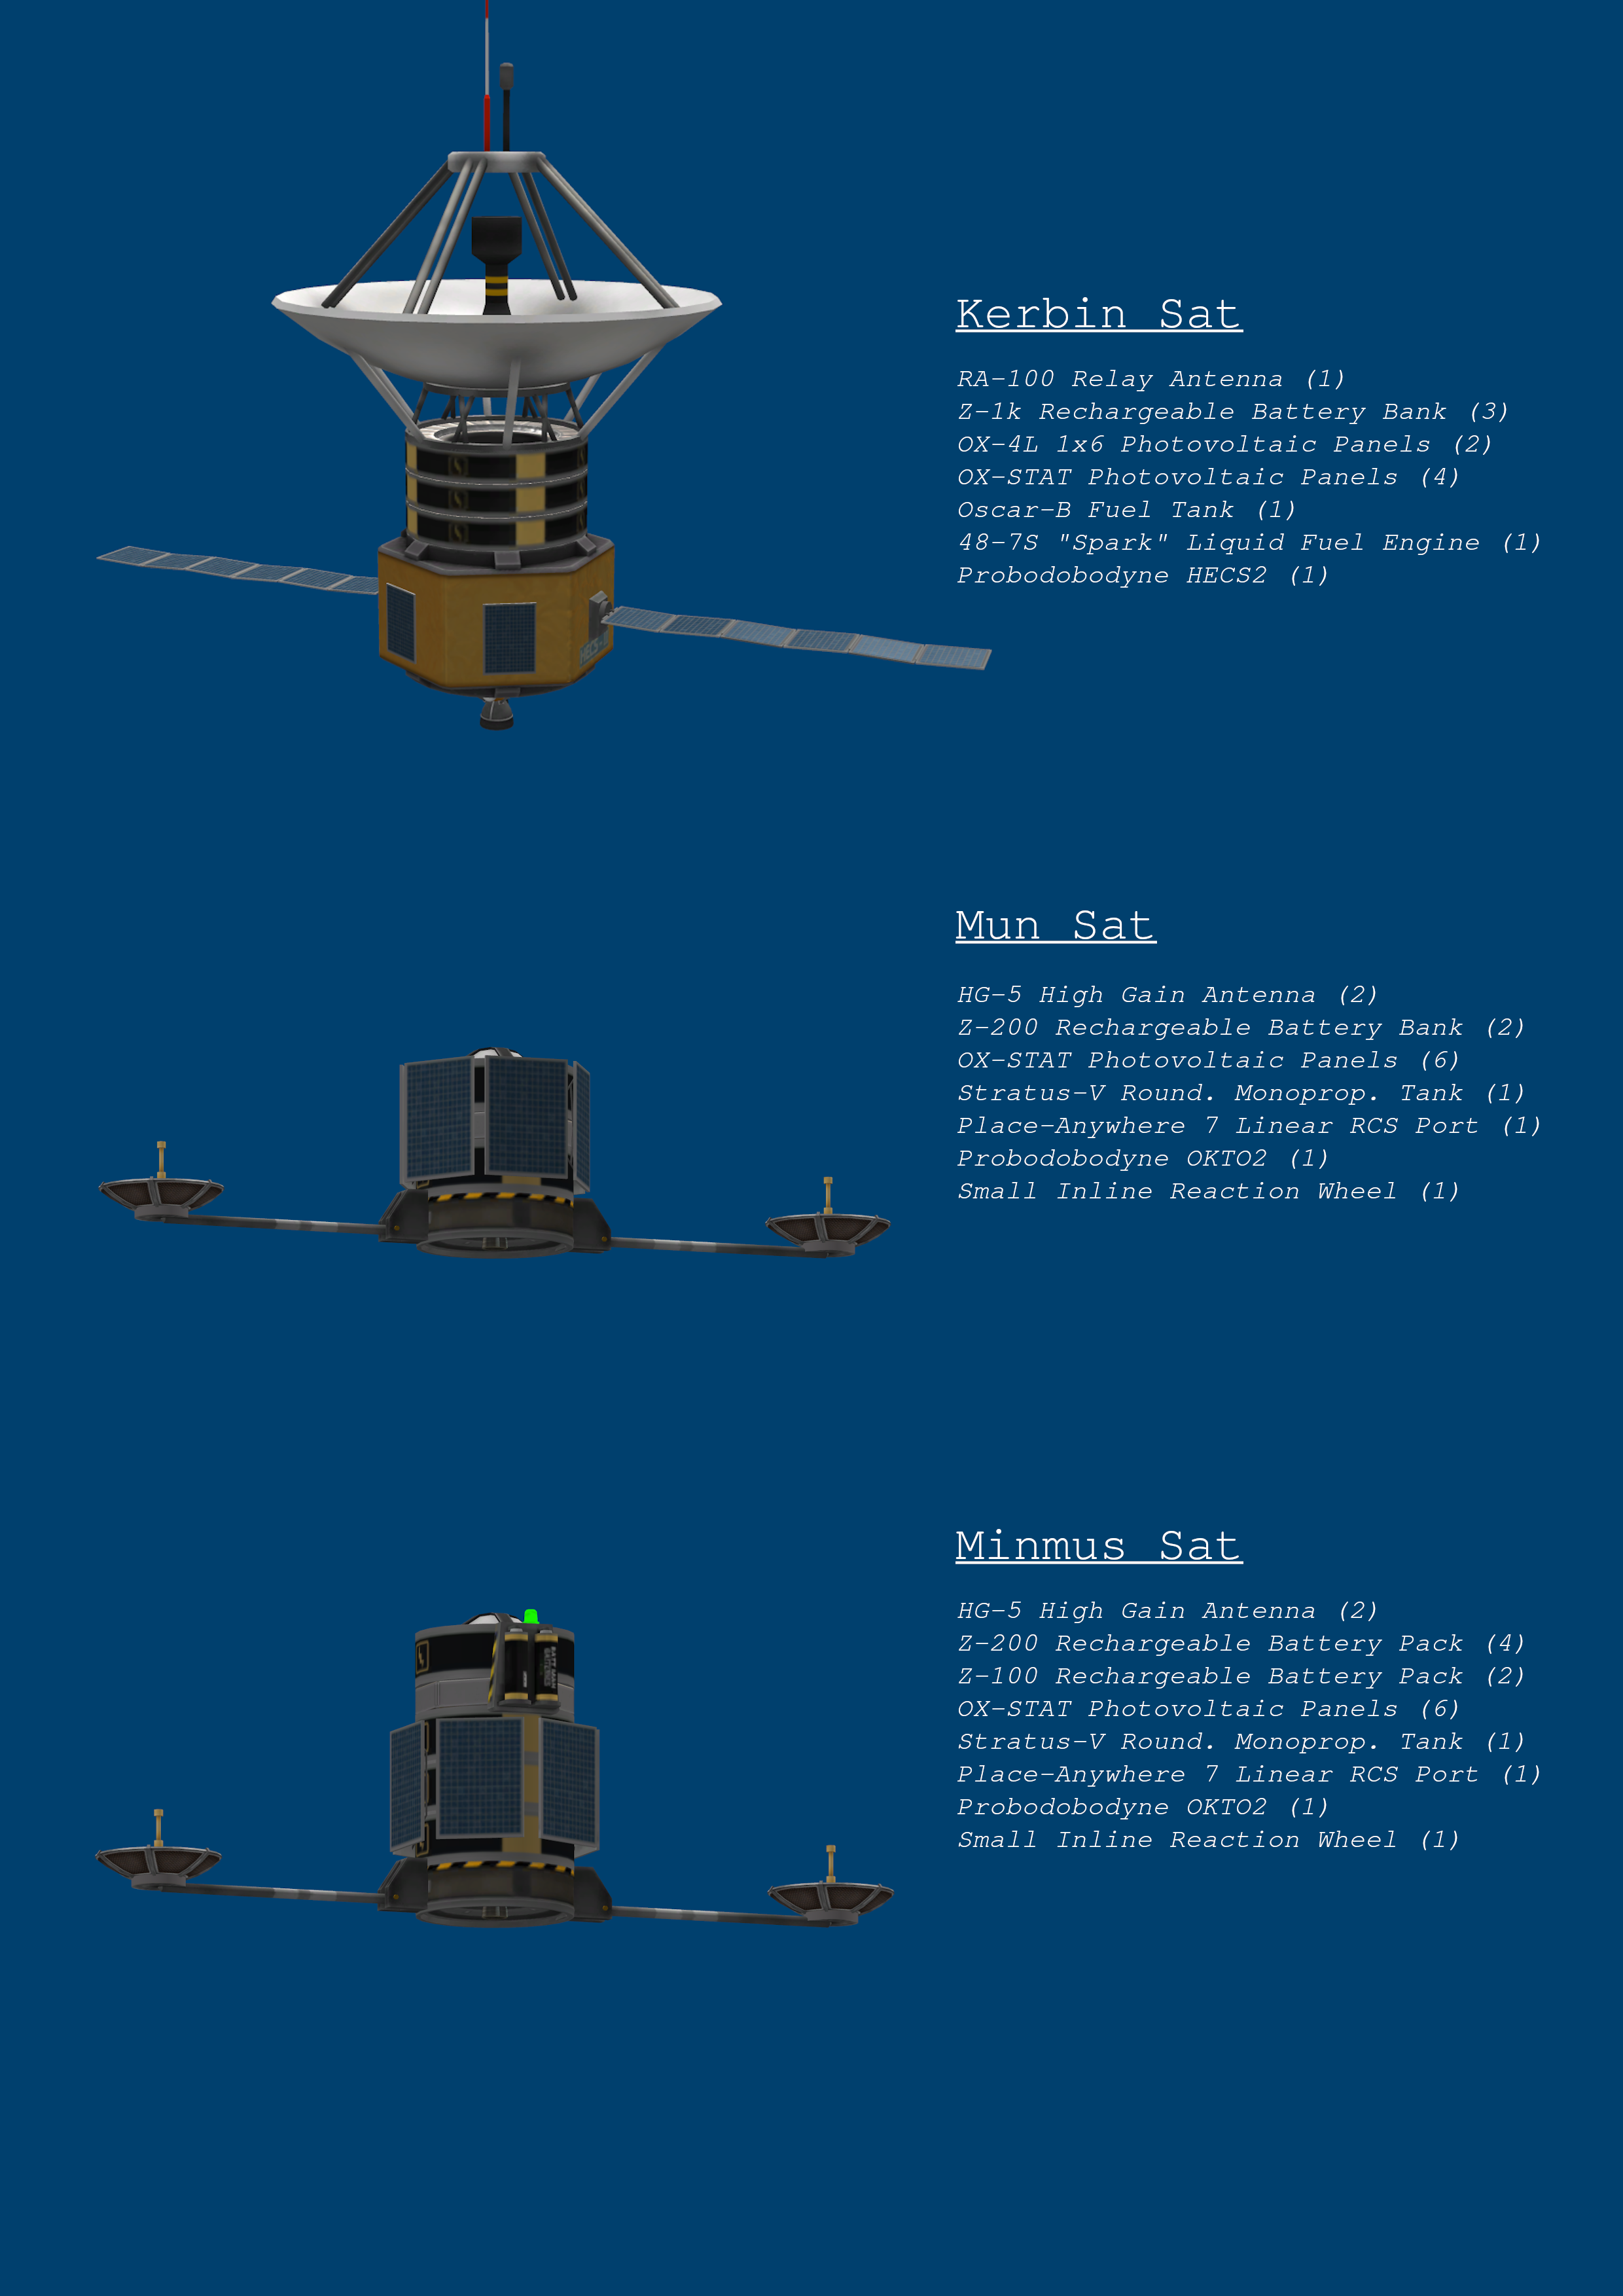
\includegraphics[width=\paperwidth,height=\paperheight]{blueprints/Sats}}
\linebreak 

\thispagestyle{empty}
\vspace*{-4cm}
\noindent\makebox[\textwidth]{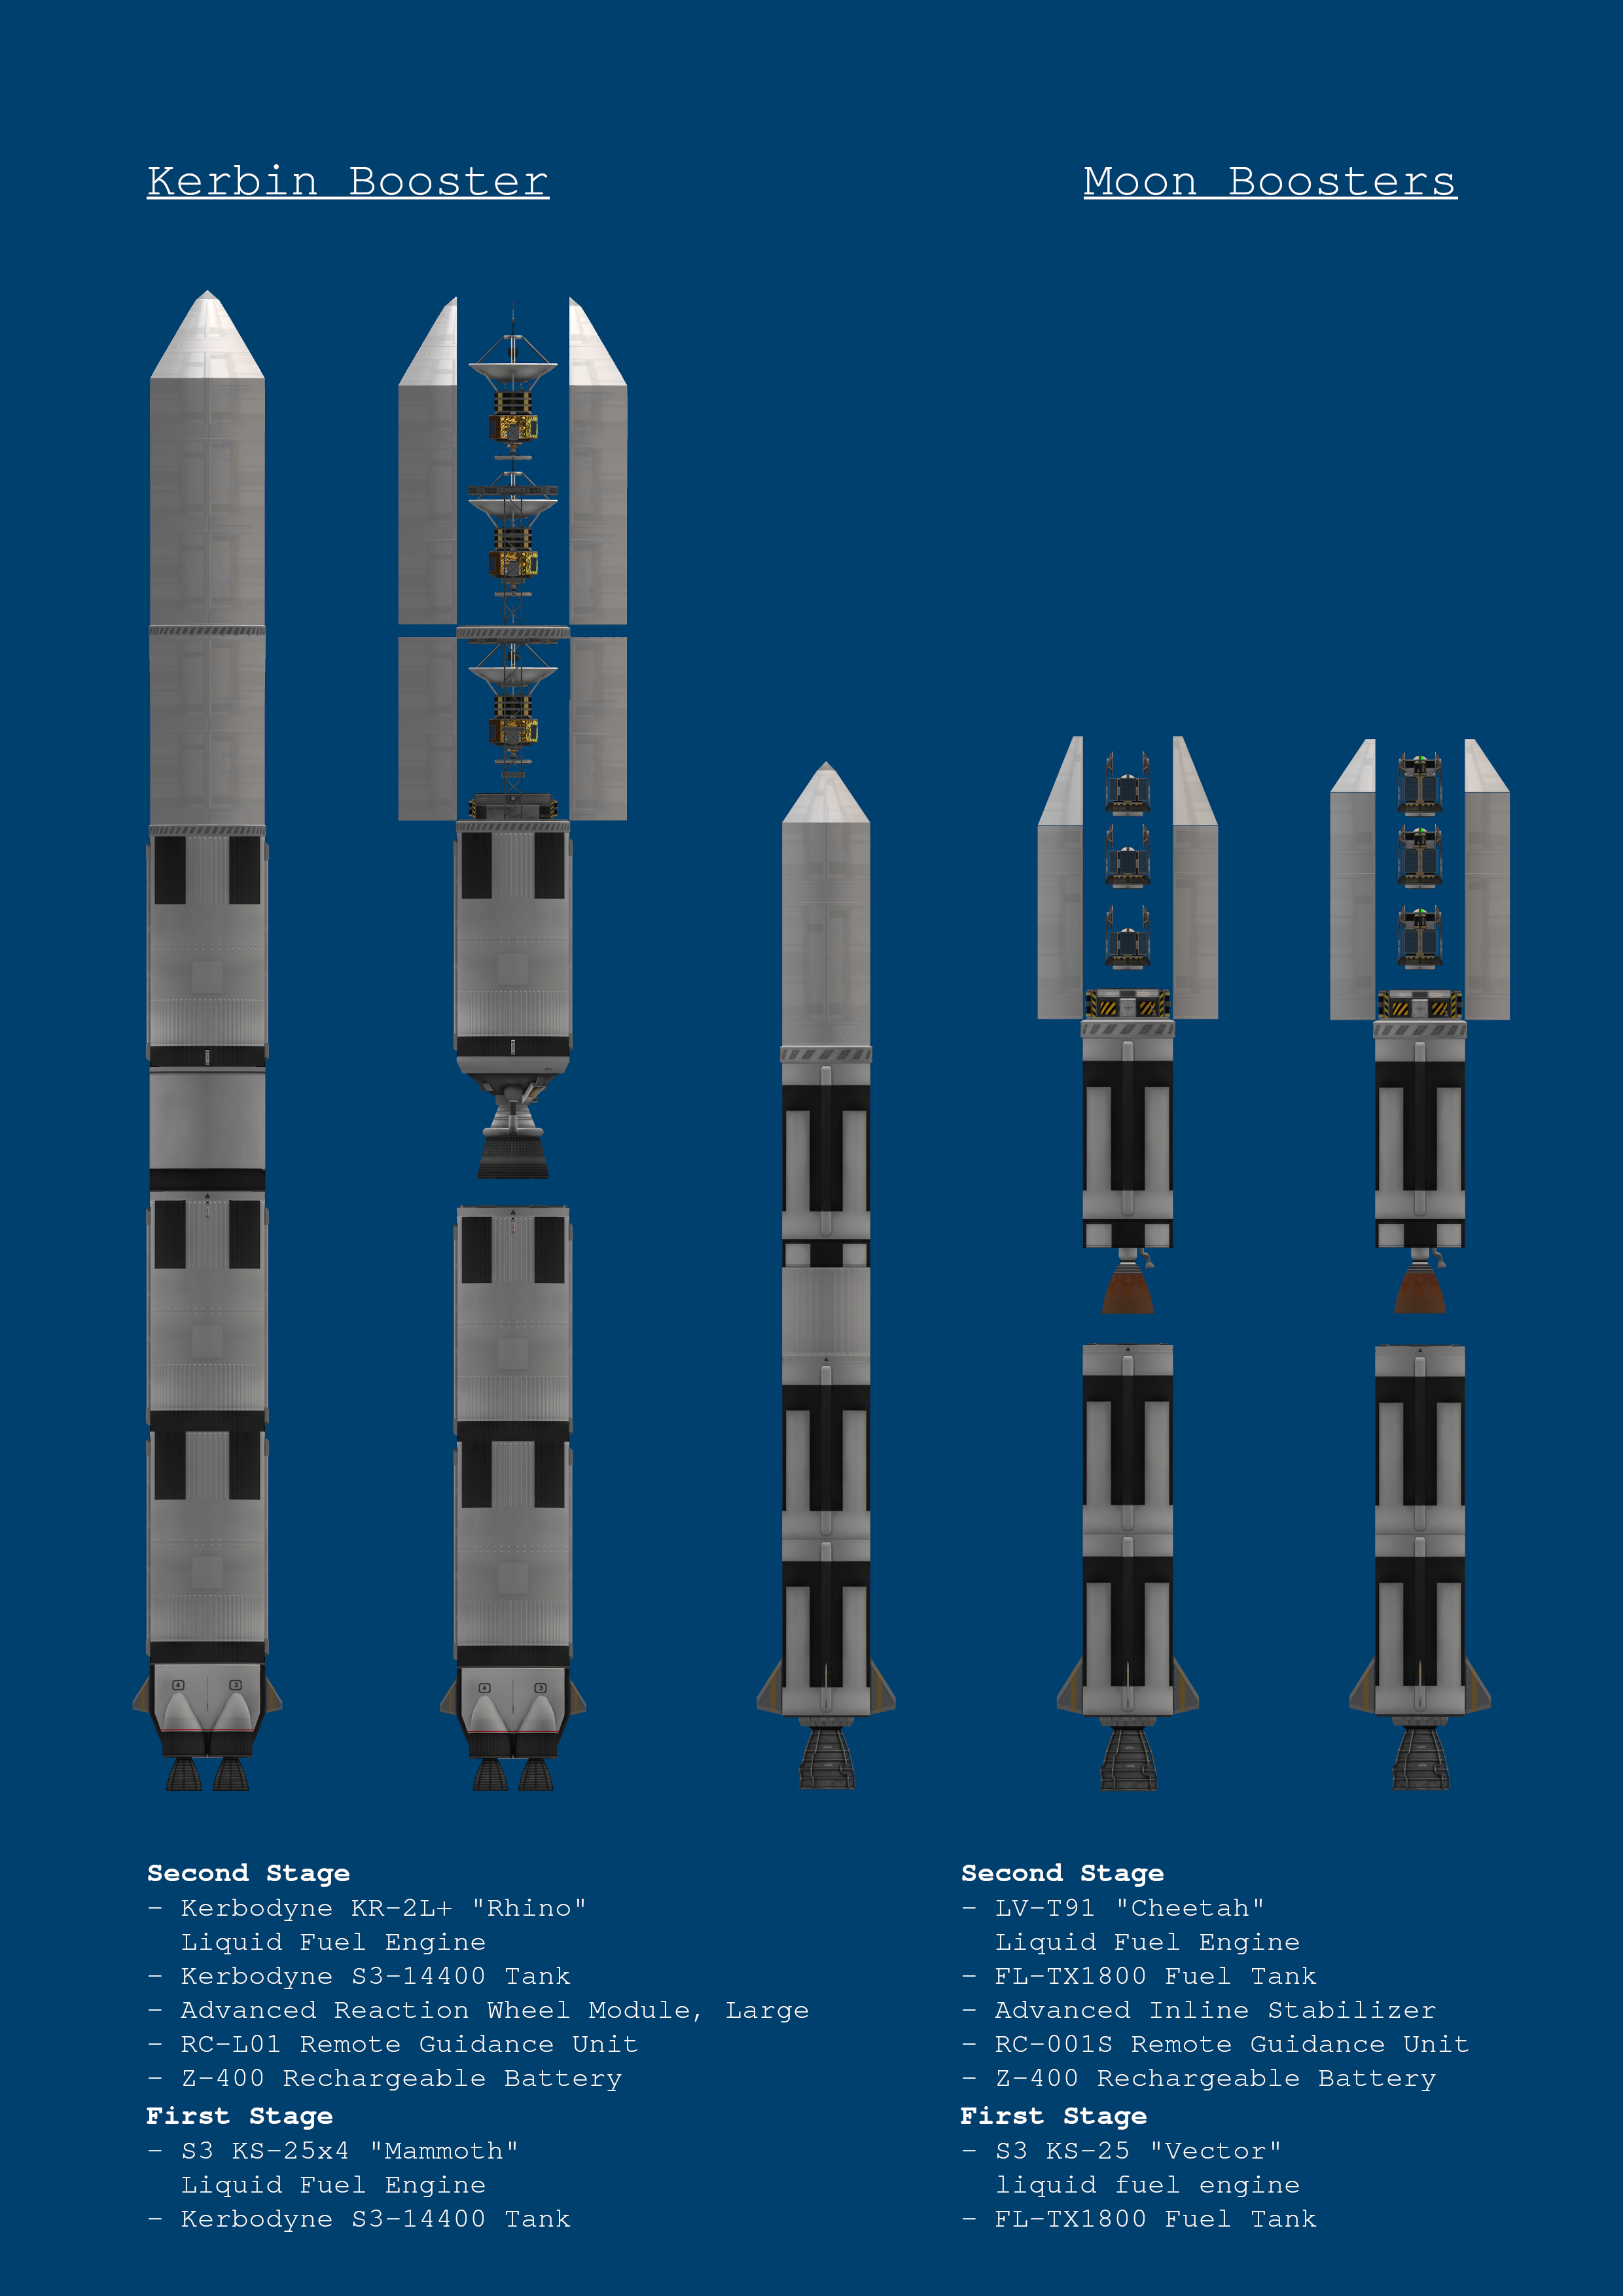
\includegraphics[width=\paperwidth,height=\paperheight]{blueprints/Rockets}}

\section*{Helper Tools}
Launch Window Planner:
\begin{itemize}
  \item \url{https://ksp.olex.biz/}
  \item \url{https://alexmoon.github.io/ksp/}
\end{itemize}
Delta-V Planner:
\begin{itemize}
\item \url{https://13375.de/KSPDeltaVMap/}
\end{itemize}
Resonant Orbit Calculator:
\begin{itemize}
  \item \url{https://meyerweb.com/eric/ksp/resonant-orbits/}
\end{itemize}
KSP Wiki Collection:
\begin{itemize}
\item \url{https://wiki.kerbalspaceprogram.com/wiki/Calculation_tools}
\end{itemize}
Addons:
\begin{itemize}
\item \url{https://spacedock.info/kerbal-space-program}
\end{itemize}


\chapter{Programming the rocket}
\section{Kerbal Operating System (kOS)}
\href{https://ksp-kos.github.io/KOS/}{kOS} is a community project by the Kerbal Space Program fanbase. It's basically an autopilot that you have to write for yourself. The mod introduces a few original parts into the game, of which at least one has to be put onto the vessel in order for it to work. Each part consists of a ``scriptable control system'' and a limited storage medium. Also keep in mind that the control chip will require additional power.\\
\linebreak 
The File-Extention for Kerboscript is always ``ks'', for example ``launch.ks''.
When opening the kOS-console in the simulator, one can then switch to the ``harddrive'' of the spacecraft by typing
\begin{code}
SWITCH TO 1.
\end{code}
\linebreak 
\emph{1} stands for the vessel and \emph{0} for the Kerbal Space Center. Because it seems unrealistic for the rocket to be always controled by the KSC, most players will transfer their script to the rocket before launching.
\begin{code}
list.
\end{code}
\linebreak 
shows the scripts that lie on the active harddrive. Keep in mind that the period at the end of an instruction is part of the syntax. Without it you will only receive error messages.
\begin{code}
COPYPATH("0:launch", "").
\end{code}
\linebreak 
copies the script ``launch.ks'' from the harddrive \emph{0} (KSC) onto the active harddrive (here \emph{1}).
\begin{code}
RUN launch. // or else
RUNPATH("launch").
\end{code}
\linebreak 
both start the script. The ``runpath'' method is simply a newer version.
The following lines of code allow for the use of additional parameters set afterwards by the user.
\begin{code}
runpath("launch",90,90000,True). // or else
run launch(90,90000,True).
\end{code}
\linebreak 
The parameter \textbf{90} stands for the compass direction of rotation ``east'', \textbf{90000} for the target orbit height in meters and \textbf{True} for an if statement (Action Group 5), because the script is supposed to be used for different rocket types, which requires the ability to use slightly different settings. \\

For the beginning I want to suggest the tutorial-series by CheersKevin - \href{https://www.youtube.com/playlist?list=PLb6UbFXBdbCoCm1e65qfDOCdK_qIBtX3D}{kOS for Newbies}.
Even suitable for future programmers! Not only can you launch rockets with those scripts, but also drones and even Airplanes.
Two very impressive examples see here: \href{https://youtu.be/f4SytD3xR0k}{HoverBot drone}, \href{https://youtu.be/oAzGwSFi9Qg}{SpaceX Falcon Heavy}.\\


\section{Reaching LEO - Low Earth Orbit}
Reaching the first stable orbit is always a challenge, here as well as in the real world. Apart from the gravitational pull, the rocket also has to fight aerodynamics and even with heat and
g-force, if you reach a too high velocity in too low of an altitude. Furthermore the rocket has to be balanced by positioning the ``center of lift'' below the ``center of mass''. So just like a dart. Of course it helps a lot that most engines have the ability to ``gimble'' - that is, they can rotate the nozzle into multiple directions.
In this way they can balance the rocket without the need of wings. In the real world you also want to pay attention to the weather in high altitudes. That is because in some heights, winds can reach high speeds of a few 100km/h, which is enough to split a rocket in half. Additionally there are also risks of lightning strikes because in differently charged air layers the rocket might act as a lightning rod. This in turn could potentially damage onboard circuits. Apollo 12 was victim to two such lightning strikes but was lucky insofar as it didn't create any permanent damage.\\

In you ever watched a rocket launch, then you might have noticed that the rocket didn't just fly straight up, but that it began to tilt sideways after just a few seconds. This is called the ``pitching maneuver''.\\
But why are rockets doing that?\\

The only reason why an object can stay in orbit is because it's parallel velocity to the surface is greater than the attraction in the direction of the planet. In this case the object will miss the earth while being pulled towards it, because it's speed is so fast that at the point, at which the planet has pulled the object 50 meters downwards, the curvature of the earth will also have ``made the ground 50 meters lower''.
Back to the rocket..\\
At low altitudes the rocket is constantly being decelerated by the atmosphere. Therefore one would normally assume that it would be the best option to leave the atmosphere as early as possible by flying straight up until it's in space. Following that, the rocket now only needs to generate speed parallel to the surface. The problem is that it normally takes a lot of time to reach the required speed of about 8km/s. In other words, you have to fly really high to have enough time left in order to reach orbital velocity. You might already have noticed that this method wastes quite a lot of energy as the vertical speed isn't what makes one stay in orbit. That's why people decided to use a curved trajectory which begins vertically and becomes horizontal over time.\\
\emph{Again: The rocket only goes ``up'' to get out of the atmosphere. If the rocket was standing on the surface of the moon, then it would only have to accelerate sideways. The only constraint might be the height of the mountains or the power of the engine (thrust to weight ratio)}.\\

%\pagebreak 
\subsection{kOS Gravity Turn}
\begin{lstlisting}[language=C, caption=launch.ks]
parameter compass is 90, finalApoapsis is 80000, fairingOrEscape is True.

SET targetPitch TO 90. //LAUNCH
SET mnvTime TO 0. //CIRCULATE
SET throttleTime TO 0. //CIRCULATE

function main {
  CLEARSCREEN.
  print "compass heading is " + compass + "degrees".
  print "finalApoapsis is " + finalApoapsis + "m".
  print "fairingOrEscape on AG5 is " + fairingOrEscape.

  doLaunch().
  doAscent().
  until apoapsis > finalApoapsis {
    doAutoStage().
    if targetPitch < 1 {
      set targetPitch to 1.
    }
  }
  doShutdown().
  doCirculate().
  print "script exited.".
}

// LAUNCH:

function doSafeStage {
  wait until stage:ready.
  stage.
  print "staging.".
}

function doLaunch {
  PRINT "Counting down:".
  FROM {local countdown is 5.} UNTIL countdown = 0 STEP {SET countdown to countdown - 1.} DO {
    PRINT "..." + countdown.
    WAIT 1.
  }
  lock THROTTLE to 1.
  doSafeStage().
  lock steering to heading(90, 90, 270).
}

function doAscent {
  set targetDirection to compass.
  set targetRoll to 0.
  wait until verticalSpeed >= 60.
  print "pitching maneuver started.".
  lock targetPitch to 1.48272E-8 * ship:altitude^2 - 0.00229755 * ship:altitude + 90.
  lock THROTTLE TO MAX(0.55, (1/90) * targetPitch).
  lock steering to heading(targetDirection, targetPitch, targetRoll).
}

function doAutoStage {
  if not(defined oldThrust) {
    declare global oldThrust to ship:availablethrust.
  }
  if ship:availableThrust < (oldThrust - 10) {
    doSafeStage(). wait 1.
    set oldThrust to ship:availablethrust.
  }
}

function doShutdown {
  lock THROTTLE to 0.
  // lock steering to prograde + R(0,0,270).
  lock steering to prograde.
  print "shutting down and holding prograde.".
}

// CIRCULATE:

function doCirculate {
  wait until ship:altitude > 70005.
  if fairingOrEscape {
    PRINT "AG5 on.".
    set AG5 to True.
    WAIT 0.5.
  }
  set mnvDeltaV to maneuverDeltaV().
  // parameter utime, radial, normal, prograde.
  local mnv is node(TIME:SECONDS + ETA:APOAPSIS, 0, 0, mnvDeltaV).
  add mnv. //addManeuverToFlightPlan
  set mnvTime to maneuverBurnTime(mnv).
  set startTime to TIME:SECONDS + ETA:APOAPSIS - (mnvTime / 2).
  set throttleTime to startTime + mnvTime - 0.3.
  //warpto(startTime - 40). //your choice whether to uncomment or not
  wait until time:seconds > startTime - 30.
  lock steering to mnv:burnvector.
  wait until time:seconds > startTime.
  lock THROTTLE to 1.
  wait until isManeuverComplete(mnv).
  lock THROTTLE to 0.
  lock steering to prograde.
  remove mnv. //removeManeuverFromFlightPlan
  print "burn finished.".
  WAIT 1. //For steering to settle down a bit
  unlock all.
  SET SHIP:CONTROL:PILOTMAINTHROTTLE TO 0.
}

function maneuverDeltaV {
  local kerbinRadius is Body:RADIUS.
  local my is constant:G * Kerbin:Mass.
  local r is SHIP:APOAPSIS + kerbinRadius.
  local a is Orbit:SEMIMAJORAXIS.
  local Vf is sqrt(my / r).  // The Velocity of any object in finalOrbit
  local Vi is sqrt(my * ((2/r) - (1/a))). // The Velocity at apoapsis
  local dV is Vf - Vi.  // Velocity-Difference from one orbit to the other.

  print "calculated dV: " + CEILING(dV,2) + "m/s.".
  return dV.
}

function maneuverBurnTime {
  parameter mnv.
  local dV is mnv:deltaV:mag.
  local g0 is constant:G * Kerbin:Mass. // OR: Kerbin:Mu
  local isp is 0.

  list engines in myEngines.
  for en in myEngines {
    if en:IGNITION and not en:FLAMEOUT {
      set isp to isp + (en:isp * (en:availablethrust / ship:availablethrust)).
    }
  }

  local mf is ship:mass / constant:e^(dV / (isp * g0)).
  local fuelFlow is ship:availablethrust / (isp * g0).
  local t is (ship:mass - mf) / fuelFlow. //maneuverBurnTime

  print "maneuverBurnTime: " + CEILING(t,2) + "s.".
  return t.
}

function isManeuverComplete {
  parameter mnv.
  if time:seconds > throttleTime {
    lock THROTTLE to 0.2.
  }
  if not(defined originalVector) or originalVector = -1 {
    declare global originalVector to mnv:burnvector.
  }
  if vAng(originalVector, mnv:burnvector) > 90 {
    declare global originalVector to -1.
    return true.
  }
  return false.
}

main().
\end{lstlisting}
\begin{flushleft}
The script shown here is also available on \href{https://github.com/Tornado3P9/kOS_Collection}{GitHub}. The beginning is sometimes difficult. Nevertheless, I want to encourage you to try to write your own script. It's not that difficult. Also there are already many good examples which might help you start....for example \href{https://kos.fandom.com/wiki/KerboScript}{this page}.\\
Alternatively there is the mod \href{https://forum.kerbalspaceprogram.com/index.php?/topic/151340-19x-smart-parts-continued/}{Smart Parts} by linuxgurugamer, for which you don't even need to know how to program. I myself often use this mod in combination, where kerboscript handles the launch and circulation burn and the smart parts stage the fairing and other things that might differ from one rocket to the other.\\
The following script just executes the next maneuver node on the active vessel's orbit. Cheers to \href{https://www.youtube.com/playlist?list=PLb6UbFXBdbCoCm1e65qfDOCdK_qIBtX3D}{CheersKevin}.
\end{flushleft}


\section{Next maneuver}
\begin{lstlisting}[language=C, caption=mnv.ks]
//--------------
//  MANEUVER:
//--------------
set mnvTime to 0.
set throttleTime to 0.

function executeManeuverNode {
  local mnv is nextNode.
  set startTime to calculateStartTime(mnv).
  set throttleTime to startTime + mnvTime - 0.3.
  //warpto(startTime - 40). //your choice whether to uncomment or not
  wait until time:seconds > startTime - 30.
  lock steering to mnv:burnvector. //lockSteeringAtManeuverTarget
  wait until time:seconds > startTime.
  lock throttle to 1.
  UNTIL isManeuverComplete(mnv){
    doAutoStage().
  }
  lock throttle to 0.
  remove mnv. //removeManeuverFromFlightPlan
  print "script exited.".
}

// STAGING:

function doSafeStage {
  wait until stage:ready.
  stage.
  print "staging.".
}

function doAutoStage {
  if ship:availableThrust = 0 {
    doSafeStage().
  }
}

// MANEUVER:


function calculateStartTime {
  parameter mnv.
  print "Node in: " + round(mnv:eta) + "s, DeltaV: " + round(mnv:deltav:mag) + "m/s.".
  set mnvTime to maneuverBurnTime(mnv).
  return time:seconds + mnv:eta - mnvTime / 2.
}

function maneuverBurnTime {
  parameter mnv.
  local dV is mnv:deltaV:mag.
  local g0 is ship:Body:MU.
  local isp is 0.

  list engines in myEngines.
  for en in myEngines {
    if en:IGNITION and not en:FLAMEOUT {
      set isp to isp + (en:isp * (en:availablethrust / ship:availablethrust)).
    }
  }

  local mf is ship:mass / constant():e^(dV / (isp * g0)).
  local fuelFlow is ship:availablethrust / (isp * g0).
  local t is (ship:mass - mf) / fuelFlow.

  print "maneuverBurnTime: " + round(t) + "s.".
  return t.
}

function isManeuverComplete {
  parameter mnv.
  if time:seconds > throttleTime {
    lock throttle to 0.2.
  }
  if not(defined originalVector) or originalVector = -1 {
    declare global originalVector to mnv:burnvector.
  }
  if vAng(originalVector, mnv:burnvector) > 90 {
    declare global originalVector to -1.
    return true.
  }
  return false.
}

executeManeuverNode().
\end{lstlisting}

For decoupling the satellites from their rocket one could use a timer that uses the orbital period as basis. The satellite could then activate it's engine when the apoapsis or the start time has been reached.\\

\noindent
{\color{black} \rule{\linewidth}{0.1mm} }


\chapter{Orbital Mechanics Crash Course}
\section{Vis-Viva Equation}
\hypertarget{visviva}{Calculating} the $\Delta v$ budget for a \href{https://forum.kerbalspaceprogram.com/index.php?/topic/83437-illustrated-tutorial-for-orbital-rendezvous/}{Hohmann Transfer} (\href{https://imgur.com/a/DmGTv}{Hohmann Transfer}).
\begin{equation}
\label{eq:visviva1}
\Delta v_{1} = \sqrt{\frac{\mu}{r_{1}}} \left( \sqrt{\frac{2r_{2}}{r_{1}+r_{2}}}-1 \right)
\end{equation}
\begin{equation}
\label{eq:visviva2}
\Delta v_{2} = \sqrt{\frac{\mu}{r_{2}}} \left( 1-\sqrt{\frac{2r_{1}}{r_{1}+r_{2}}} \right)
\end{equation}

$\Delta v_{1}$ stands for the cost of the first burn that raises one side of the orbit to the height of the target orbit.

$\Delta v_{2}$ stands for the cost of the second burn that will be executed at the intersection with the target orbit and will transfer the current orbit towards the target orbit.

Together they give the $\Delta v$ budget of each spacecraft that transfers from one circular orbit into another circular orbit. \\
Instead of $\sqrt{\frac{2r}{r_{1}+r_{2}}}$ one can also write $\sqrt{\frac{r}{a}}$. The original fraction divided by two shows the radius as the numerator and the semimajor axis as the denominator.\\
For learning the origin of this formular I suggest the video by \href{https://youtu.be/7AkakB5TOSw}{Mike Aben}. Or perhaps on Wikiwand: \href{https://www.wikiwand.com/en/Hohmann_transfer_orbit}{Hohmann transfer orbit}.

\medskip
The \href{https://en.wikipedia.org/wiki/vis-viva_equation}{Vis-viva equation} for the \hypertarget{velocityatorbitposition}{instantaneous velocity of a body} that is located on an orbit around another body is called:
\begin{equation}
v = \sqrt{GM \left( \frac{2}{r} - \frac{1}{a} \right) }
\end{equation}
where:
\begin{itemize}
\item $v$ is the relative speed of the two bodies
\item $r$ is the distance between the two bodies
\item $a$ is the length of the semi-major axis ($a > 0$ for ellipses, $a \rightarrow \infty$ for parabolas, and $a < 0$ for hyperbolas)
\item G is the gravitational constant
\item M is the mass of the central body
\end{itemize}
The product of GM can also be expressed as the standard gravitational parameter using the Greek letter $\mu$.\\
If $a = r$ for all $r$, then the Keplerian orbit will degenerate to a circular orbit; the body always has got the same distance $r$ from it's center of gravity and accordingly always the same \textbf{orbital velocity}
\begin{equation}
v_{1} = \sqrt{\frac{G(m+M)}{r}} = \sqrt{\frac{\mu}{r}}
\end{equation}
The formula for \textbf{escape velocity} can be obtained from the Vis-viva equation by taking the limit as $a$ approaches $\infty$:
\begin{equation}
v_{2} = \sqrt{\frac{2G(m+M)}{r}} = v_{1}\cdot\sqrt{2}
\end{equation}
If the orbital velocity is equal to $v_{2}$, then the orbit isn't a closed circle anymore, but rather a parabola. At even higher speeds, while $r$ being the same, the path becomes a hyperbola and the semi-major axis $a$ becomes (formally) negative.

You will sometimes see the mass \textit{m} of the spacecraft being omitted. This, of course, can easily be explained, as it's mass compared to that of the planets is so insignificantly small that an effect is just not measureable. If for instance you plan to circle an Asteroid, then of course you will have to account for that also. (Not in the game though. Only the sun, planets and moons have gravity there.)


\section{Other Stuff}
Also insteresting to note: Until an \textbf{altitude} of somewhere around 500km there is still a lot of atmosphere left, enough to brake out and deorbit satellites over time. In the past there were only spy-satellites in very low orbits. 340km is already the minimum height that a satellite can hold without deorbiting.
But even the ISS, with it's 400km is not that high, if you think about it. When the space shuttles were still flying, the ISS was even lower. On this altitude, the residual atmosphere is still so high that the ISS has to raise it's orbit about once a year. There is a wonderful animation \href{https://qz.com/296941/interactive-graphic-every-active-satellite-orbiting-earth/}{QUARTZ - every active satellite orbiting earth} that illustrates this pendulum motion very well.\\
And another three-dimensional representation of all near earth objects you can find at \href{http://stuffin.space/}{stuffin.space}. You can even hide certain satellites and for instance only display GPS satellites. By the way, GPS satellites usually live inside the \href{https://en.wikipedia.org/wiki/Medium_Earth_orbit}{Medium Earth Orbit (MEO)}.

In case of \textbf{SpaceX Starlink}, it's satellites only stay in orbit for as long they still have fuel in their tanks. That makes maintenance of those networks a little bit more difficult, but you have the certainty that any defect satellites will deorbit automatically after 5 years and that no space debree will ever be left behind.
Unlike other satellite providers who also use ion thruster, SpaceX decided to use Krypton as reaction mass instead of Xenon, which is more common. Another name you may find is Hall-effect thruster (HET).

\textbf{Factor of safety} often lies between 1.1 and 1.25, as is the case for ULA's rockets.
It expresses how much stronger a system is than it needs to be for an intended load.
For spacecrafts this factor is usually very low, because every millimeter that you add to the thickness of a tank wall, will probably add many kilos or even tons of extra weight, which in turn requires a stronger engine and more fuel...which adds more weight...which reduces the payload mass that the rocket can bring with it into space.\\
In contrast, a tractor can have a much higher FoS, because stability and sheer power are much more important  than are in this case weight or speed. See also \href{https://youtu.be/o0fG_lnVhHw}{HOW ROCKETS ARE MADE (Rocket Factory Tour - United Launch Alliance) - Smarter Every Day 231}.

%%%%%%%%%%%%%%%%%%%%%%%%%%%%%%%%%%%%%%%%%%%%%%%%

\listoffigures

\lstlistoflistings

%%%%%%%%%%%%%%%%%%%%%%%%%%%%%%%%%%%%%%%%%%%%%%%%

%\begin{thebibliography}{}  % Literaturverzeichnis 
%\bibitem[xx, 1900]{}
% ().
%\emph{} 
%\end{thebibliography}

\clearpage
\begin{center}
	\colorbox{ghell}{%
		\parbox{0.8\linewidth}{
		Hereby, I declare that I have composed the presented paper independently on my own and without any 				other resources than the ones indicated. All thoughts taken directly or indirectly from external 				sources are properly denoted as such.
		\par
		\begin{center}
		
\includegraphics[width=0.8\textwidth]{bilder/sign}
		\end{center}
		\hspace*{0.8cm}Place, Date \hfill Signature\hspace*{0.8cm}
		}
	}
\end{center}

\end{document}
